\documentclass[12pt, a4paper]{book}

\usepackage{fancyhdr}
\usepackage[left=4cm, right=4cm, top=4cm, bottom=4cm]{geometry}
\usepackage[utf8]{inputenc}
\usepackage[table]{xcolor}
\usepackage{hyperref}
\usepackage{multirow}
\usepackage{amsmath}
\usepackage{enumitem}
\usepackage{graphicx}
\usepackage{booktabs}
\usepackage{subcaption}
\usepackage[justification=centering]{caption}
\usepackage{xepersian}

\DeclareMathOperator*{\argmax}{argmax}
\DeclareMathOperator*{\argmin}{argmin}
\newcolumntype{L}{>{$}l<{$}} % math-mode version of "l" column type

\newcommand{\coursetitle}{شبکه‌های عصبی}
\newcommand{\doctitle}{تمرین ششم}
\newcommand{\name}{محمدرضا غفرانی}
\newcommand{\studentno}{400131076}
\newcommand{\todaydate}{\today}

\settextfont{XB Kayhan}
\setlatintextfont{Times Newer Roman}

\pagestyle{fancy}
\lhead{\textbf{\doctitle}}
\chead{\name}
\rhead{\todaydate}

\begin{document}

\begin{flushleft}
    \name \\
    \studentno \\
    \todaydate
\end{flushleft}

\begin{center}
    \huge
    \textbf{\coursetitle}
    \break
    \large
    \doctitle
\end{center}

% suppress the fancy header on the first page only
\thispagestyle{plain}

\section*{سوال یک}

هما‌‌ن‌طور که می‌دانیم هر دو سلول \lr{LSTM} و \lr{GRU} برای ساختن شبکه‌های بازگشتی استفاده می‌شوند. هر دو این شبکه‌ها نیز برای
بهبود عملکرد واحد \lr{RNN} عرضه شده‌اند. در ادامه جزئیات بیشتری از این دو مدل تشریح می‌شود.

واحد \lr{LSTM} از سه دروازه\LTRfootnote{gate} اصلی تشکیل شده است: دروازه ورودی، دروازه صرف‌نظر\LTRfootnote{forget} و دروازه
خروجی. هر یک از این دروازه‌ها وظیفه خاصی به عهده دارد. دروازه ورودی وظیفه تصمیم‌گیری درباره حجم اطلاعات وارد
شده به واحد \lr{LSTM} دارد. دروازه صرف‌نظر همان‌طور که از نام‌ آن پیداست وظیفه تصمیم‌گیری درباره میزان دانش
که باید دور ریخته شود را به عهده دارد. دروازه خروجی نیز خروجی واحد \lr{LSTM} را بر اساس دانش کسب شده
تولید می‌کند. در شکل \ref{lstm_architecture} نمایی از واحد \lr{LSTM} آورده شده است.

\begin{figure}[h]
    \centering
    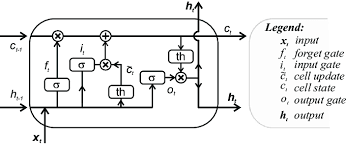
\includegraphics[width=0.55\linewidth]{images/q1/lstm.png}
    \caption{ساختار واحد \lr{LSTM}}
    \label{lstm_architecture}
\end{figure}

واحد \lr{GRU} از دو دروازه تشکیل شده است: دروازه به‌روزرسانی\LTRfootnote{update} و دروازه بازنشانی\LTRfootnote{reset}.
عملکرد دروازه بازنشانی مشابه دروازه صرف‌نظر در واحد \lr{LSTM} است. این واحد وظیفه تصمیم‌گیری در رابطه با فراموش کردن
دانشی که مدل تا به حال یادگرفته را به عهده دارد. واحد به‌روزرسانی نیز مسئول تصمیم‌گیری در خصوص میزان دانشی است
که مدل به واحد بعدی منتقل می‌کند. همان‌طورکه مشاهده می‌شود عملکرد این دروازه بسیار شبیه عملکرد دروازه خروجی در واحد
\lr{LSTM} است. در شکل \ref{gru_architecture} نمونه‌ای از واحد \lr{GRU} آورده شده است.

\begin{figure}[h]
    \centering
    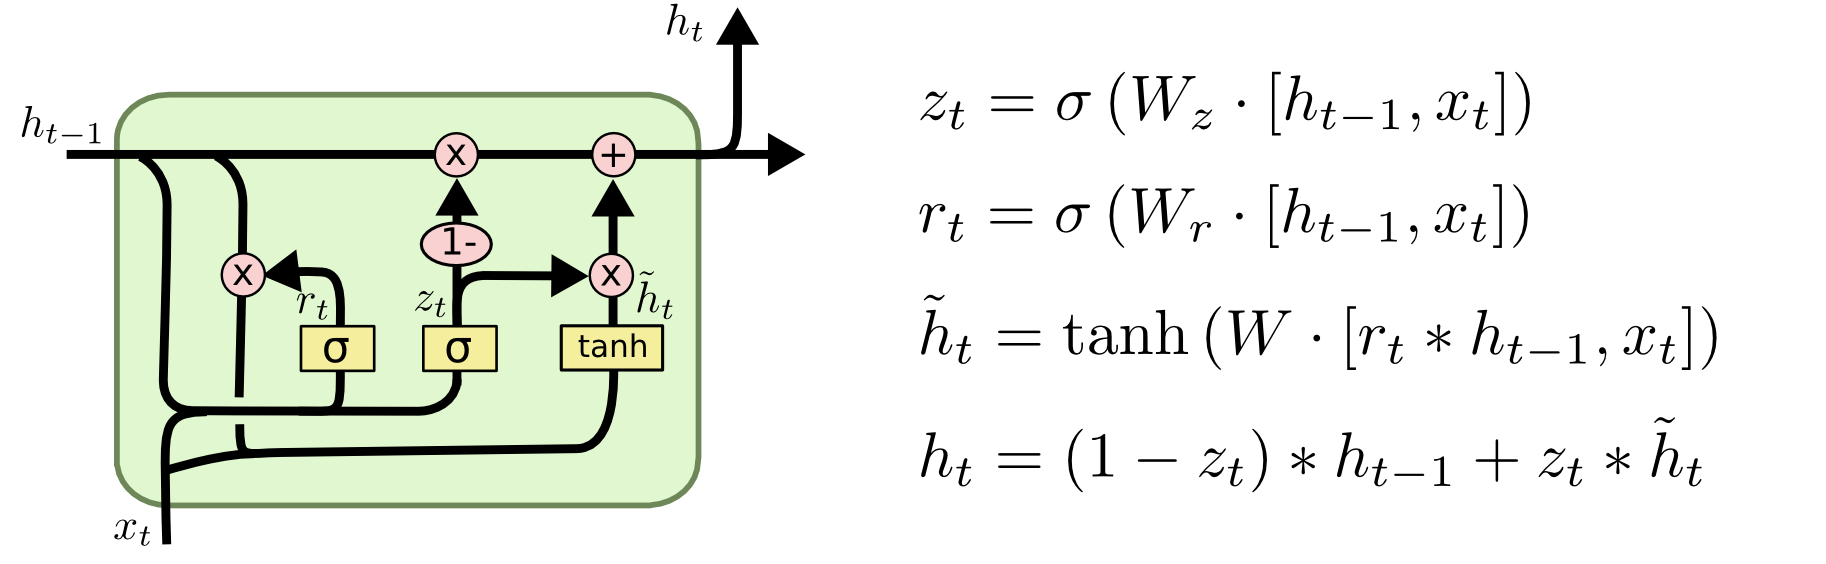
\includegraphics[width=0.8\linewidth]{images/q1/gru.png}
    \caption{ساختار واحد \lr{GRU}}
    \label{gru_architecture}
\end{figure}

با توجه به توضیحات داده شده مشخص است که واحد \lr{GRU} تعداد پارامتر‌های کمتری نسبت به واحد \lr{LSTM} دارد.
این مسئله باعث می‌شود قدرت شبکه \lr{GRU} در مقایسه با \lr{LSTM} کم‌تر شود. از طرفی بیشتر شدن قدرت باعث افزایش
واریانس شده و در نتیجه احتمال بیش‌برازش واحد \lr{LSTM} رو داده‌های ورودی بیشتر می‌شود. بنابراین اگر تعداد داده‌ها
و ویژگی‌ها زیاد باشد بهتر است از مدل \lr{LSTM} استفاده شود، در غیر این صورت استفاده از شبکه عصبی \lr{GRU} منطقی‌تر
به نظر می‌رسد. با همه‌ی این تفاسیر توصیه‌ای که در استفاده از مدل‌های \lr{LSTM} و \lr{GRU} در حل مسائل می‌شود این
است که هر دو مدل برای حل مسئله امتحان شود.

\section*{سوال دو}

در ابتدا توضیحاتی در رابطه با پیش‌پردازش انجام شده بر روی داده‌ها توضیحاتی داده می‌شود.

در قدم اول فایل‌های \lr{csv} که در اختیار ما قرار داده شده بود با استفاده از کتابخانه \lr{pandas} بارگیری
می‌شود. در این میان بعضی از فایل‌ها داده خاصی نداشته و خالی هستند بنابراین این فایل‌ها دور ریخته می‌شوند.
سپس سطر‌های مشترک موجود در جداول با استفاده از فیلد \lr{\texttt{<DTYYYYMMDD>}} ادغام و مرتب می‌شود. پس از ادغام فایل‌‌ها
داده‌های یکسال اخیر را در نظر گرفته و باقی داده‌ها را حذف می‌کنیم. همچنین ستون‌هایی که تعداد مقادیر غیرتکرار آن‌ها
کم‌تر از ۲ است را حذف می‌کنیم. استدلال ما برای حذف این ستون‌ها این است که ستون‌هایی که تعداد مقادیر غیرتکراری آن‌ها
بسیار کم است، بیشتر از آن که به مدل پیش‌بینی بهتر کمک کنند، باعث گمراهی آن می‌شوند. با اعمال این شرط ستون‌های
\lr{\texttt{<TICKER>}}، \lr{\texttt{<COL12>}} و \lr{\texttt{<COL13>}} از مجموعه دادگان حذف می‌شوند.

در نهایت لازم است که تعیین کنیم آیا شاخص در یک روز مشخص صعودی بوده یا خیر. برای این کار از تفاضل \lr{close}
هر روز نسبت به روز قبل استفاده می‌کنیم. اگر مقدار این تفاضل مثبت بود یعنی شاخص مثبت بوده و با مقدار
یک نشان می‌دهیم در غیر این صورت مقدار شاخص منفی بوده و با عدد صفر نمایش می‌دهیم.

علاوه بر اقدامات بالا، کار‌های دیگری نیز برای پیش‌پردازش داده‌ها صورت گرفته است:

\begin{itemize}
    \item دو سطر از داده‌ها در بعضی از ستون‌ها بدون مقدار بودند. با توجه به آن که تعداد کل داده‌هایی که در اختیار داریم
    کم است، این دو سطر را دور نریختیم و میانگین سطر‌های قبل و بعد از سطر مذکور را به عنوان مقدار آن خانه خالی در
    نظر گرفتیم.
    \item برای آن که به نتیجه بهتری برسیم با استفاده از \lr{\texttt{MinMaxScaler}} ارائه شده توسط کتابخانه \lr{sklearn}
    داده‌های هر ستون را با توجه به کمینه و بیشینه آن ستون، به بازه $(0,1)$ نگاشت می‌کنیم.
    \item برای آن که داده‌ها ماهیت سری زمانی داشته باشند، داده‌های هر ۱۰ روز متوالی را با یک برچسب به مدل دادیم.
    منظور از برچسب صعودی یا نزولی بودن شاخص در روز ۱۱ام پس از این ۱۰ روز است.
\end{itemize}

پس از پیش‌پردازش داده‌ها نوبت به تقسیم داده‌ها به مجموعه داده‌های آموزش، ارزیابی و آزمون می‌رسد. ما در این مرحله
تلاش می‌کنیم داده‌ها را به نحوی تقسیم کنیم که تا جای امکان هر سه مجموعه داده متعادل باشند. پس از تقسیم داده‌ها
در مجموعه داده آموزشی، ارزیابی و آزمون به ترتیب حدود ۵۷، ۵۶ و ۵۵ درصد داده‌ها را داده‌های با برچسب یک تشکیل می‌دهند.
این درصد‌ها بیانگر آن هستند که توزیع برچسب‌ها در هر سه مجموعه داده یکسان و متعادل هستند.

پیش از ارائه نتایج نیز لازم است نکاتی در رابطه با چگونگی استخراج نتایج بیان شود.

\begin{itemize}
    \item نتایج با ۵ مرتبه آموزش و ارزیابی ارائه شده است. بنابراین می‌توان انتظار داشت که با تکرار آزمایش‌ها
    همین نتایج دوباره به دست آید.
    \item برای به دست آوردن نتایج مقادیر مختلف برای پارامتر‌های زیر بررسی شده و نتایج بر اساس بهترین پارامتر‌ها
    گزارش شده است.
    \begin{itemize}
        \item نرخ یادگیری. برای نرخ یادگیری مقادیر $0.01$، $0.001$ و $0.001$ امتحان شده است.
        \item تابع بهینه‌ساز. توابع بهینه‌ساز \lr{Adam} و \lr{SGD} برای رسیدن به جواب بهینه بررسی شده است.
    \end{itemize}
    \item تعداد گام یادگیری مدل بر روی ۳۰۰ تنظیم شده است.
    \item با توجه به زیاد بودن تعداد گام یادگیری برای جلوگیری از بیش‌برازش، از یک \lr{Early Stopping Callback} با مقدار صبر ۲۰ بر
    روی خطای داده‌های ارزیابی استفاده شده است.
\end{itemize}

نتایجی که مدل \lr{LSTM} می‌رسد در جدول \ref{lstm_single_layer} آمده است.
این نتایج با استفاده از بهینه‌ساز \lr{Adam} و با نرخ یادگیری $0.001$
به دست آمده است.

\begin{latin}
    \begin{table}[h]
    \centering
    \caption{\rl{نتایج عملکرد مدل \lr{LSTM} با تعداد مختلف ابعاد لایه مخفی}}
    \label{lstm_single_layer}
    \rowcolors{2}{teal!40}{teal!10}
    \begin{tabular}{l|l|l|l}
        \rowcolor{teal!50}
        \# of hcells & Train Accuracy & Validation Accuracy & Test Accuracy \\
        \hline
        8 & 0.6 & 0.57 & 0.56 \\
        32 & 0.61 & 0.59 & 0.56 \\
        64 & 0.62 & 0.57 & 0.58 \\
        256 & 0.62 & 0.57 & 0.57 \\
        512 & 0.59 & 0.57 & 0.55 \\
    \end{tabular}
    \end{table}
\end{latin}

نتایج عملکرد مدل \lr{GRU} با استفاده از بهینه‌ساز \lr{Adam} و نرخ یادگیری $0.001$ نیز در جدول \ref{gru_single_layer}
مشاهده می‌شود.

\clearpage

\begin{latin}
    \begin{table}[h]
    \centering
    \caption{\rl{نتایج عملکرد مدل \lr{GRU} با تعداد مختلف ابعاد لایه مخفی}}
    \label{gru_single_layer}
    \rowcolors{2}{teal!40}{teal!10}
    \begin{tabular}{l|l|l|l}
        \rowcolor{teal!50}
        \# of hcells & Train Accuracy & Validation Accuracy & Test Accuracy \\
        \hline
        8 & 0.62 & 0.6 & 0.53 \\
        32 & 0.63 & 0.58 & 0.56 \\
        64 & 0.61 & 0.58 & 0.57 \\
        256 & 0.65 & 0.57 & 0.58 \\
        512 & 0.65 & 0.56 & 0.56 \\
    \end{tabular}
    \end{table}
\end{latin}

همان‌طور که مشاهده می‌شود، عملکرد هر دو شبکه \lr{LSTM} و \lr{GRU} با افزایش تعداد نورون‌ها در لایه‌های مخفی
اندکی بهتر می‌شود. اما با ادامه افزایش تعداد نورون‌ها عملکرد شبکه افت می‌کند. به عبارت دیگر با افزایش تعداد نورون‌ها شبکه
بهتر توانسته است الگوی کلی داده‌ها را شناسایی کرده و یاد بگیرد.
اما این روند با افزایش بیش‌ از حد نورون‌های لایه مخفی عکس شده و شبکه الگوهای بسیار جزئی از
داده‌های آموزشی را یاد گرفته که در نتیجه نتوانسته روی داده‌های ارزیابی و آزمون به خوبی عمل کند. به عبارت بهتر
با افزایش تعداد نورون‌ها پدیده بیش‌برازش رخ داده است. البته همان‌طور که پیش‌تر ذکر شد ما از یک \lr{Early Stopping Callback}
برای جلوگیری از بیش‌برازش مدل استفاده کرده‌ایم. اگر از این \lr{callback}
استفاده نمی‌شد تاثیر بیش‌برازش مدل بسیار واضح‌تر می‌بود.

با توجه به جدول، عملکرد هر دو شبکه \lr{LSTM} و \lr{GRU} تا حد زیادی شبیه یکدیگر هستند. معیاری که برای انتخاب
بهترین عملکرد در نظر می‌گیریم عملکرد هر دو مدل روی داده‌های آزمون است. هر دو این شبکه‌ها توانسته‌اند به دقت
58 درصد روی داده‌های آزمون دست یابند. اما هر یک از این دو شبکه با تعداد متفاوت نورون‌های لایه مخفی. شبکه \lr{LSTM}
با توجه به پیچیدگی زیاد‌تری که دارد به تعداد نورون‌های کمتری نیاز داشته است تا به این عملکرد برسد در حالی که
شبکه \lr{GRU} برای آن که به این دقت برسد، به تعداد بسیار بیشتری نورون نیاز داشته است. نکته مشابهی در هنگامی
که تعداد نورون‌های لایه مخفی کم است مشاهده می‌شود. هنگامی که تعداد نورون‌های لایه مخفی هر دو شبکه ۸ است، شبکه \lr{LSTM}
عملکرد بهتری را ارائه می‌دهد.

یکسان بودن بهترین عملکرد هر دو مدل را می‌توان کم بودن داده آموزشی در عین پیچیدگی آن در نظر گرفت.
به نظر می‌رسد این عملکرد یک کران بالا برای هر دو مدل باشد. چرا که هر دو مدل با تنظیم درست تعداد پارامتر‌ها
می‌توانند به آن برسند. برای آن که به نتایج بهتری از عملکرد مدل‌ها در این حالت دست پیدا کنیم حالت‌های
بسیار زیادی تست شده است. نتایج ارائه شده با استفاده از بهترین پارامتر‌ها ارائه شده است. تلاش‌هایی که
برای رسیدن به بهترین نتایج انجام شده است در ادامه آورده می‌شود. متاسفانه بیشتر این تلاش‌ها باعث بهبود مدل نشده‌اند.

\begin{itemize}
    \item استفاده از بهینه‌ساز‌های مختلف
    \item استفاده از نرخ‌های مختلف یادگیری
    \item تغییر بازه دخیل در پیش‌بینی مدل
    \item تفکیک چندباره مدل به مجموعه داده‌های آموزش، ارزیابی و آزمون و آموزش مدل بر روی آن‌ها
    \item استفاده از شاخص کل به صورت مجزا برای آموزش مدل و حذف سایر شاخص‌ها
\end{itemize}

\section*{سوال سه}

نتایج عملکرد مدل پشته‌ای حاصل از سلول‌های \lr{LSTM} در جدول \ref{lstm_stacked_layer} و نتایج مدل پشته‌ای از
واحد‌های \lr{GRU} در شکل \ref{gru_stacked_layer} دیده می‌شود. برای آموزش هر دو این شبکه‌ها از بهینه‌ساز
\lr{Adam} و نرخ یادگیری $0.0001$ استفاده شده است.

همان‌طور که مشاهده می‌شود نتایج عملکرد هر دو مدل نسبت به حالتی که تنها از یک لایه سلول بازگشتی استفاده می‌شود
اندکی بهتر است. با افزایش تعداد لایه‌های بازگشتی نیز عملکرد مدل‌ها اندکی بهبود می‌یابد. تفسیر این اتفاق آن است
این مدل‌ها بهتر می‌توانند الگوهای پیچیده موجود در داده‌ها را شناسایی کنند. در نتیجه عملکرد بهتری روی داده‌های
ارزیابی و آزمون دارند.

انتظار می‌رفت پشته‌ کردن لایه‌های بازگشتی \lr{GRU} عملکرد بهتری نسبت به \lr{LSTM} داشته باشد.
چرا که شبکه‌های \lr{GRU} از ساختار ساده‌تری برخوردار هستند بنابراین پشته‌کردن که به معنای افزایش پارامتر‌ها است،
قدرت‌ آن‌ها را به طور معقول‌تری در مقایسه با پشته‌کردن شبکه‌های \lr{LSTM} افزایش می‌دهد. به هر حال با پشته‌کردن هر دو مدل
عملکرد هر دو مدل بهبود یافته است. شاید یکی از دلایلی که باعث جلوگیری از بیش‌برازش مدل‌های پشته‌ای \lr{LSTM}
شده است، استفاده از نرخ یادگیری بسیار کم ($0.001$) در کنار \lr{Early Stopping Callback} باشد. با توجه به آن که
تعداد گام آموزشی بسیار زیاد (۳۰۰ گام) است مدل \lr{GRU} به آرامی به سمت بهتر شدن پیش می‌رود در حالی که آموزش مدل
\lr{LSTM} در همان گام‌های ابتدایی متوقف می‌شود.

\begin{latin}
    \begin{table}[h]
    \centering
    \caption{\rl{نتایج عملکرد مدل \lr{LSTM} با تعداد مختلف ابعاد لایه مخفی و تعداد پشته‌های مختلف}}
    \label{lstm_stacked_layer}
    % \rowcolors{2}{teal!40}{teal!10}
    \begin{tabular}{c|l|l|l|l}
        \rowcolor{teal!50}
        \# of stacks & \# of hcells & Train Acc & Validation Acc & Test Acc \\
        \hline
        \rowcolor{teal!10}
        & 8 & 0.63 & 0.6 & 0.6\\ \rowcolor{teal!10}
        & 32 & 0.65 & 0.6 & 0.6\\ \rowcolor{teal!10}
        & 64 & 0.64 & 0.57 & 0.6 \\ \rowcolor{teal!10}
        & 256 & 0.61 & 0.61 & 0.59 \\ \rowcolor{teal!10}
        \multirow{-5}{*}{2} & 512 & 0.65 & 0.59 & 0.58 \\ \rowcolor{teal!40} \hline
        & 8 & 0.62 & 0.62 & 0.62 \\ \rowcolor{teal!40}
        & 32 & 0.65 & 0.57 & 0.61\\ \rowcolor{teal!40}
        & 64 & 0.64 & 0.57 & 0.64 \\ \rowcolor{teal!40}
        & 256 & 0.64 & 0.6 & 0.62 \\ \rowcolor{teal!40}
        \multirow{-5}{*}{3} & 512 & 0.65 & 0.57 & 0.62\\ \rowcolor{teal!10} \hline
        & 8 & 0.64 & 0.63 & 0.61\\ \rowcolor{teal!10}
        & 32 & 0.64 & 0.67 & 0.61 \\ \rowcolor{teal!10}
        & 64 & 0.63 & 0.61 & 0.64 \\ \rowcolor{teal!10}
        & 256 & 0.64 & 0.63 & 0.63 \\ \rowcolor{teal!10}
        \multirow{-5}{*}{4} & 512 & 0.63 & 0.58 & 0.6 \\
    \end{tabular}
    \end{table}
\end{latin}

\clearpage

\begin{latin}
    \begin{table}[h]
    \centering
    \caption{\rl{نتایج عملکرد مدل \lr{GRU} با تعداد مختلف ابعاد لایه مخفی و تعداد پشته‌های مختلف}}
    \label{gru_stacked_layer}
    % \rowcolors{2}{teal!40}{teal!10}
    \begin{tabular}{c|l|l|l|l}
        \rowcolor{teal!50}
        \# of stacks & \# of hcells & Train Acc & Validation Acc & Test Acc \\
        \hline
        \rowcolor{teal!10}
         & 8 & 0.66 & 0.59 & 0.6 \\ \rowcolor{teal!10}
        & 32 & 0.64 & 0.62 & 0.61 \\ \rowcolor{teal!10}
        & 64 & 0.64 & 0.55 & 0.6 \\ \rowcolor{teal!10}
        & 256 & 0.63 & 0.59 & 0.59\\ \rowcolor{teal!10}
        \multirow{-5}{*}{2} & 512 & 0.64 & 0.57 & 0.58 \\ \rowcolor{teal!40} \hline
        & 8 & 0.62 & 0.65 & 0.6\\ \rowcolor{teal!40}
        & 32 & 0.64 & 0.63 & 0.61 \\ \rowcolor{teal!40}
        & 64 & 0.65 & 0.6 & 0.62 \\ \rowcolor{teal!40}
        & 256 & 0.65 & 0.57 & 0.64 \\ \rowcolor{teal!40}
        \multirow{-5}{*}{3} & 512 & 0.65 & 0.55 & 0.59 \\ \rowcolor{teal!10} \hline
        & 8 & 0.61 & 0.61 & 0.59 \\ \rowcolor{teal!10}
        & 32 & 0.63 & 0.63 & 0.63 \\ \rowcolor{teal!10}
        & 64 & 0.63 & 0.64 & 0.63 \\ \rowcolor{teal!10}
        & 256 & 0.62 & 0.63 & 0.6 \\ \rowcolor{teal!10}
        \multirow{-5}{*}{4}& 512 & 0.64 & 0.6 & 0.64 \\
    \end{tabular}
    \end{table}
\end{latin}

\end{document}